\subsection{Complex geometries}

\begin{frame}{Learn a regular levelset}		
    \vspace{-10pt}
    \hypersetup{
		citecolor=white,
	}

    \begin{mytheo}{\footnotesize\citep{clemot_neural_2023}\normalsize}{fem}
		If we have a boundary domain $\Gamma$, the SDF is solution to the Eikonal equation:
		
		\begin{minipage}{0.7\linewidth}
			\hspace{100pt}
			$\left\{\begin{aligned}
				&||\nabla\phi(X)||=1, \; X\in\mathcal{O} \\
				&\phi(X)=0, \; X\in\Gamma \\
				&\nabla\phi(X)=n, \; X\in\Gamma
			\end{aligned}\right.$
		\end{minipage}
		\begin{minipage}{0.25\linewidth}
			\centering
			\pgfimage[width=0.7\linewidth]{images/newlines/levelset/points_normals.png}
		\end{minipage}
		
		with $\mathcal{O}$ a box which contains $\Omega$ completely and $n$ the exterior normal to $\Gamma$.
	\end{mytheo}

    \hypersetup{
        citecolor=other,
    }

    \vspace{5pt}

    \textbf{Objective:} Move on to complex geometries by using a levelset function to

    \begin{itemize}
        \item Sample points in the domain $\Omega$ for the PINN training.
        \item Impose exactly the boundary condition in PINN \citep{Sukumar_2022}.
    \end{itemize}

    \vspace{5pt}

	\textbf{How to learn a regular levelset ?} with a PINN by \textcolor{orange}{adding a regularization term},
	\vspace{-5pt}
	\begin{equation*}
		J_{reg} = \int_\mathcal{O} |\Delta\phi|^2,
	\end{equation*}
    and a sample of boundary points that considers the \textcolor{orange}{curvature} of $ \Gamma$. \filledstar

    % Curvature
\end{frame}

\begin{frame}{Numerical results}		
    \begin{figure}[!ht] \centering
		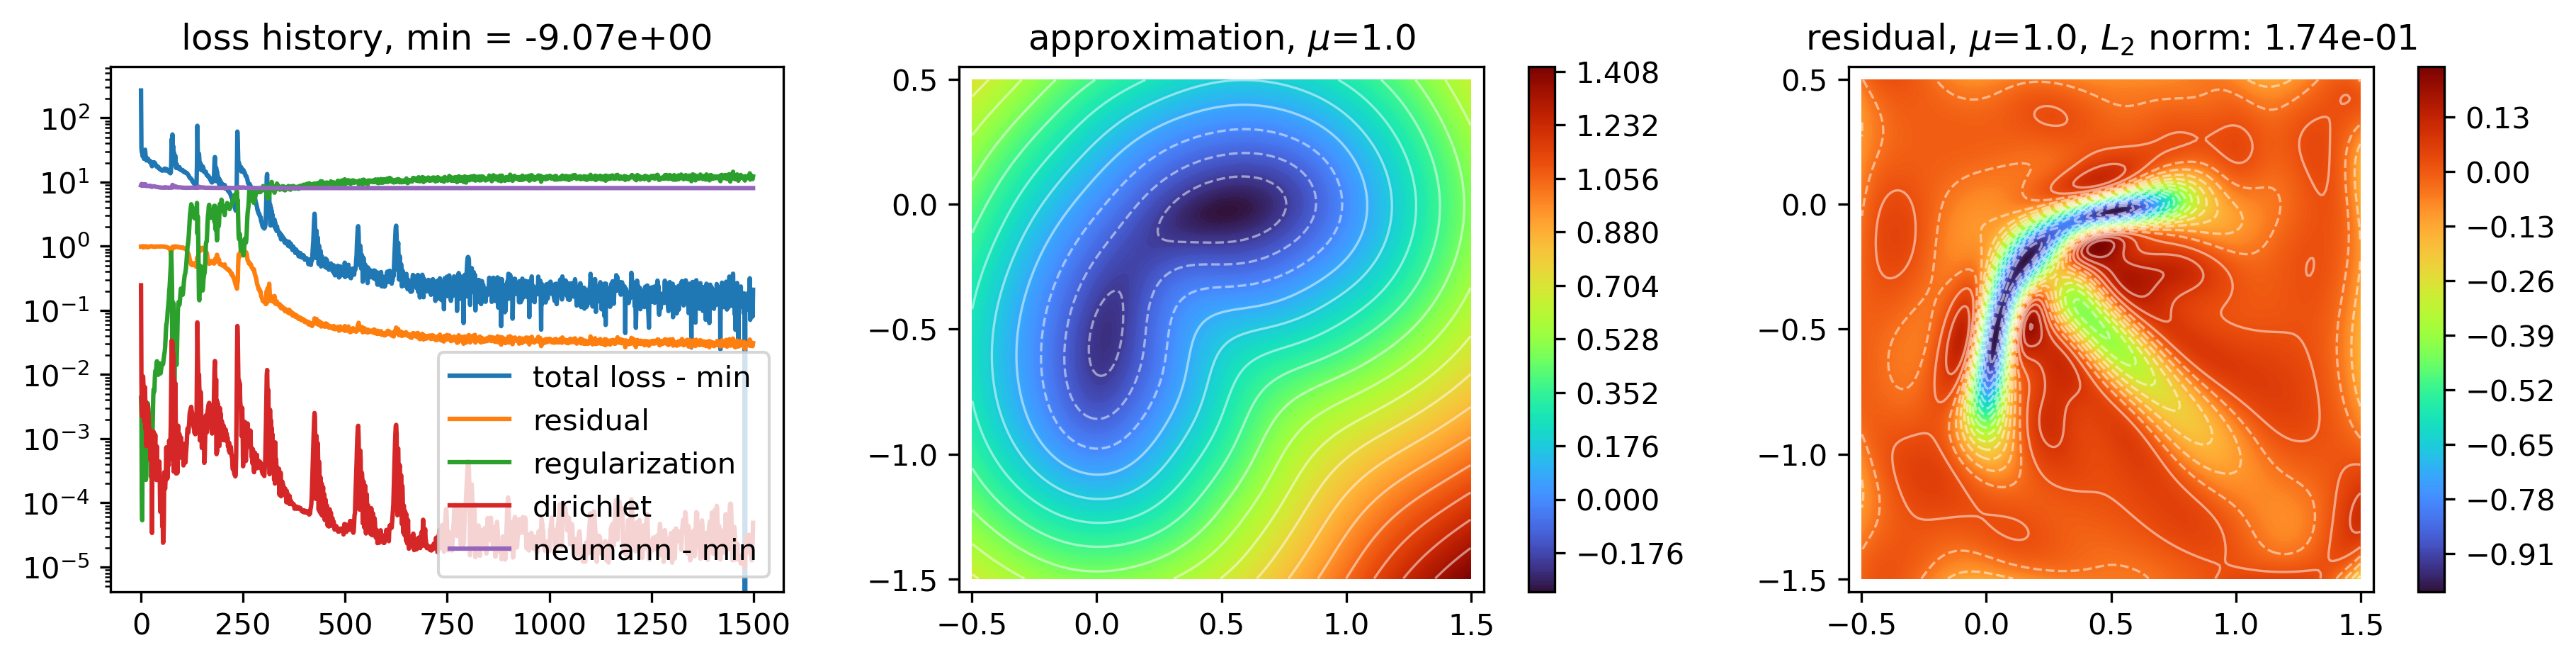
\includegraphics[width=\linewidth]{images/newlines/levelset/EikonalBean_curvature.png}

        % \vspace{10pt}

		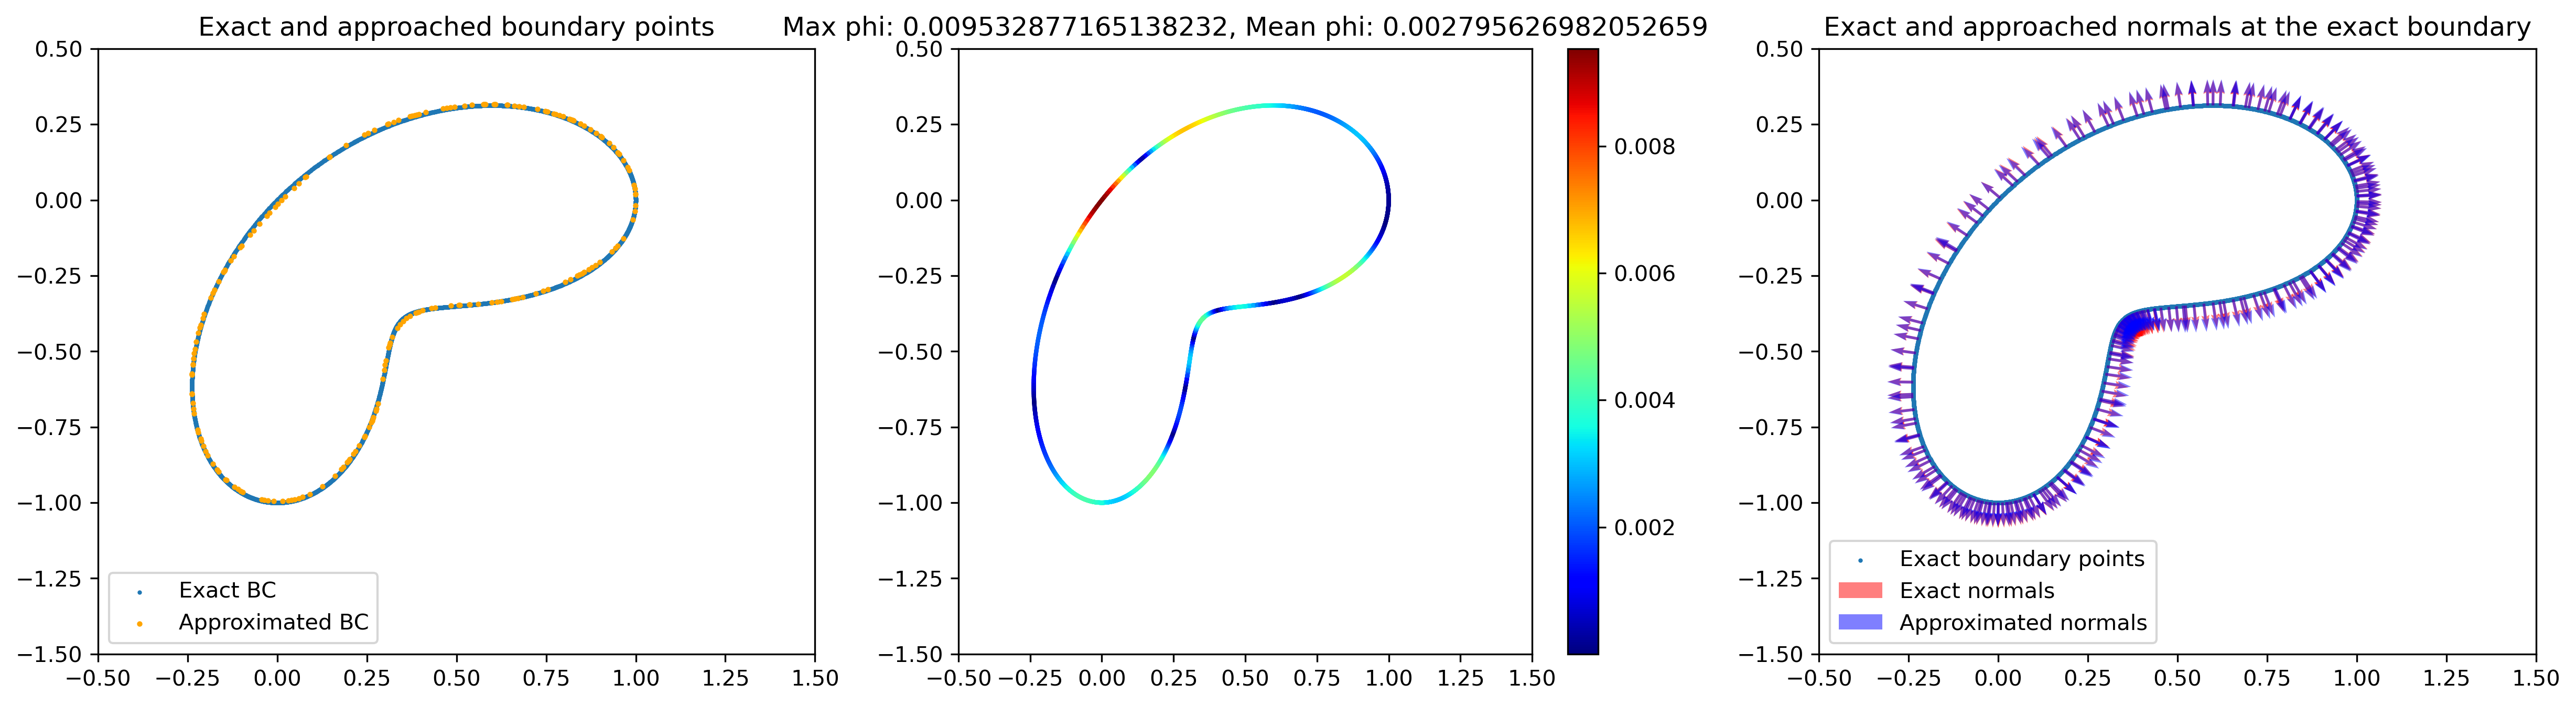
\includegraphics[width=\linewidth]{images/newlines/levelset/boundary_curvature.png}
	\end{figure}

    \vspace{-5pt}
    TODO : Ajouter résultats "Poisson on Bean" + Mettre au propre les images. 
\end{frame}

\subsection{\filledstar Posteriori error estimates}

\begin{frame}{Adaptive mesh refinement}	
    \textbf{Adaptive refinement loop} using Dorfler marking strategy. \refappendix{frame:amr} %(residual estimator)
    
    \begin{center}
        \textbf{Standard FEM}
        \vspace{2pt}

        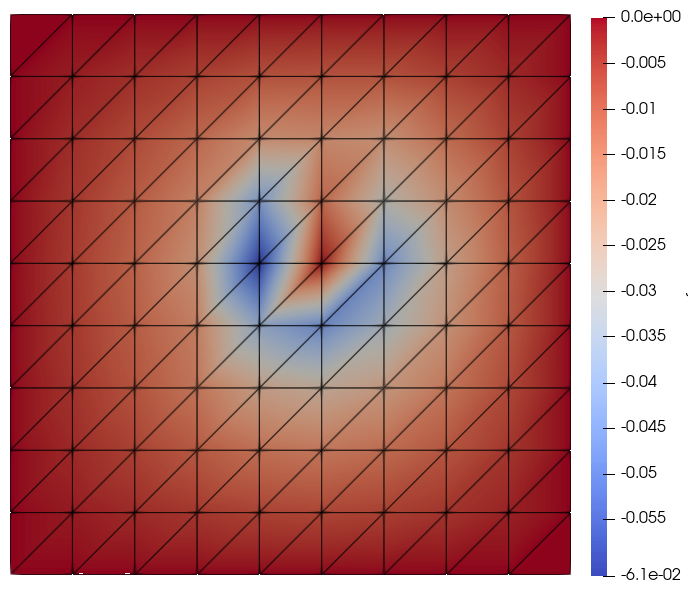
\includegraphics[width=0.2\linewidth]{images/newlines/mesh/explications/fem/u_h.png}
        \quad
        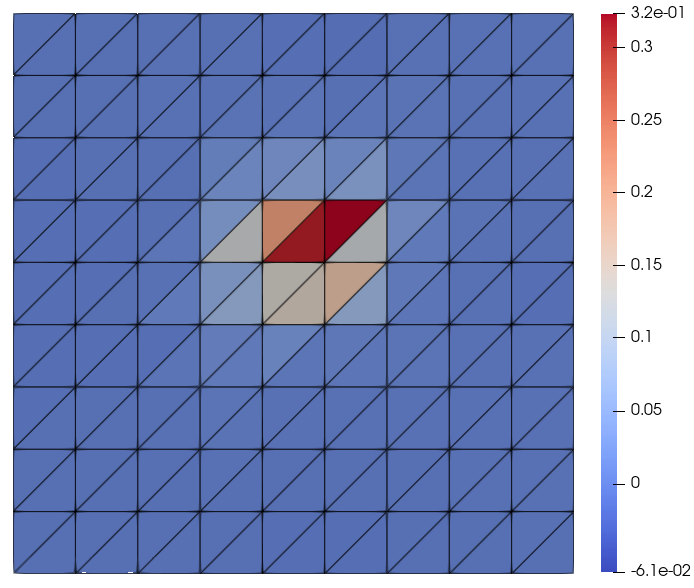
\includegraphics[width=0.2\linewidth]{images/newlines/mesh/explications/fem/eta_h.png}
        \quad
        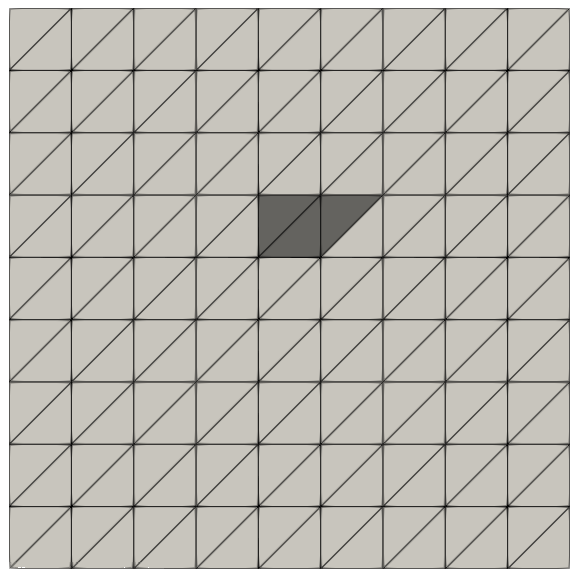
\includegraphics[width=0.17\linewidth]{images/newlines/mesh/explications/fem/marking.png}
        \qquad
        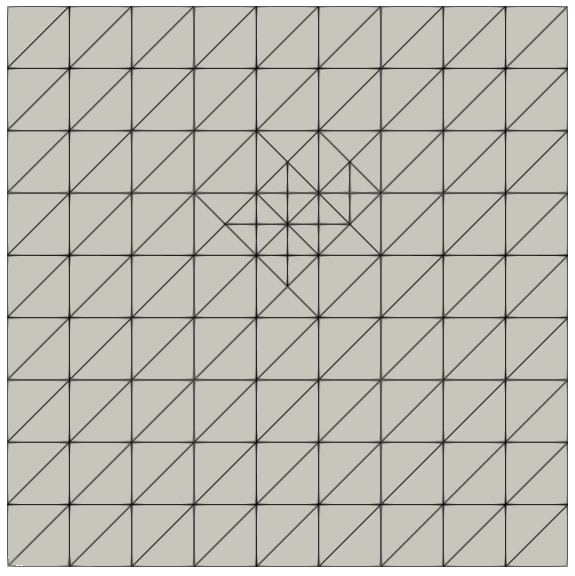
\includegraphics[width=0.17\linewidth]{images/newlines/mesh/explications/fem/refined.png}
    \end{center}

    \vspace{-10pt}
    $\cdots\hspace{1pt}\longrightarrow\hspace{8pt}
    \text{SOLVE}\hspace{18pt}\longrightarrow\hspace{6pt}
    \text{ESTIMATE}\hspace{8pt}\longrightarrow\hspace{14pt}
    \text{MARK}\hspace{14pt}\longrightarrow\hspace{8pt}
    \text{REFINE}\hspace{4pt}\longrightarrow\hspace{1pt}
    \cdots$

    \hspace{45pt}$\text{on }u_h\hspace{55pt}\eta_{res,T}$

    \vspace{8pt}
    \textbf{Local residual estimator (in $L^2$ norm):} Let $T$ be a cell of $\mathcal{T}_h$ .

    \vspace{-8pt}
    $$\eta_{res,T}^2 = h_T^4 \|\Delta u_h + f_h\|_{L^2(T)}^2 + \frac{1}{2} \sum_{E \in \partial T} h_E^2 \|[\nabla u_h\cdot n]\|_{L^2(E)}^2$$
    with $h_\bullet$ the size of $\bullet$ and considering the Poisson problem.

    % Considering the Poisson problem with Dirichlet boundary conditions.

    % (en précisant que c'est le coût du solve qui est le plus important)
\end{frame}

\begin{frame}[noframenumbering]{Adaptive mesh refinement}	
    \textbf{Adaptive refinement loop} using Dorfler marking strategy.
    
    \begin{center}
        \textcolor{red}{\textbf{Additive Approach}}
        \vspace{2pt}

        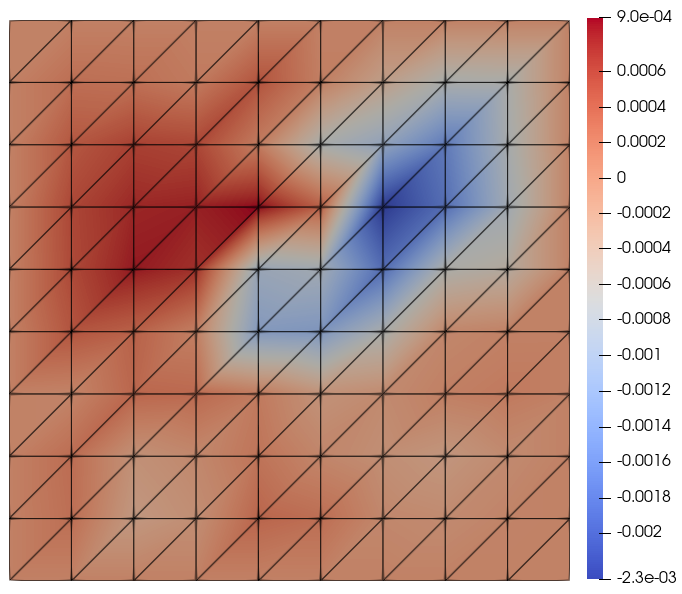
\includegraphics[width=0.2\linewidth]{images/newlines/mesh/explications/add/p_h.png}
        \quad
        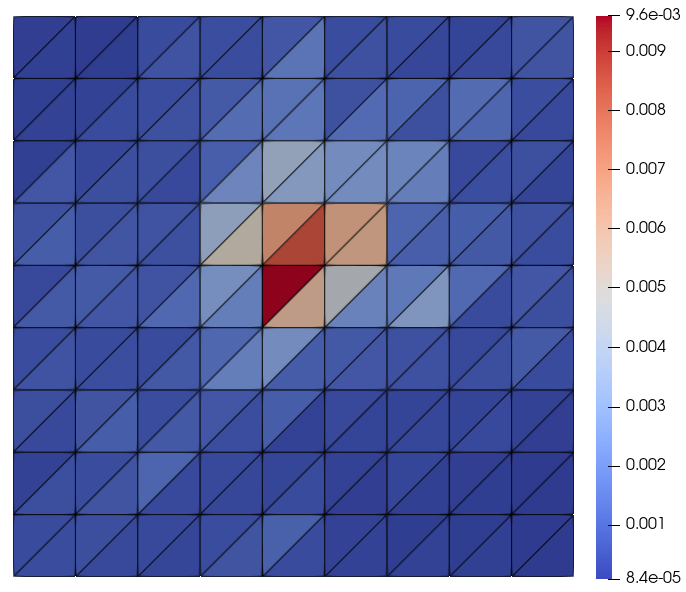
\includegraphics[width=0.2\linewidth]{images/newlines/mesh/explications/add/eta_h_add.png}
        \quad
        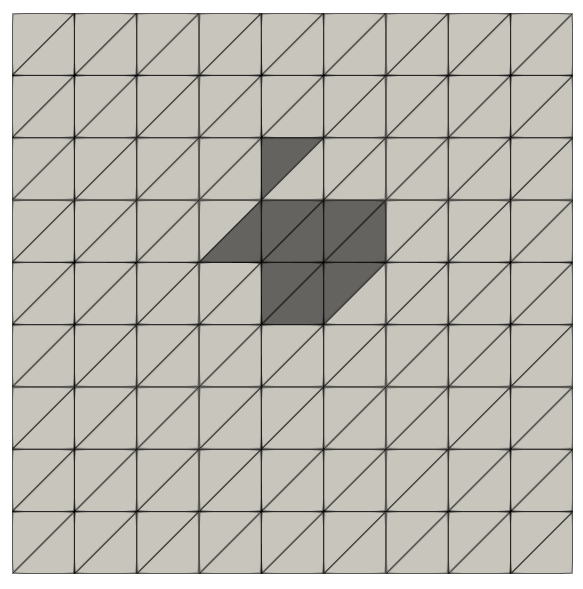
\includegraphics[width=0.17\linewidth]{images/newlines/mesh/explications/add/marking_add.png}
        \qquad
        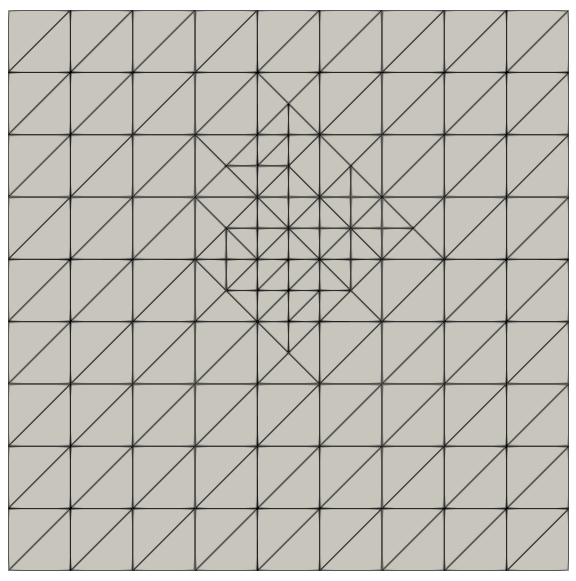
\includegraphics[width=0.17\linewidth]{images/newlines/mesh/explications/add/refined_add.png}
    \end{center}

    \vspace{-10pt}
    $\cdots\hspace{1pt}\longrightarrow\hspace{8pt}
    \text{SOLVE}\hspace{18pt}\longrightarrow\hspace{6pt}
    \text{ESTIMATE}\hspace{8pt}\longrightarrow\hspace{14pt}
    \text{MARK}\hspace{14pt}\longrightarrow\hspace{8pt}
    \text{REFINE}\hspace{4pt}\longrightarrow\hspace{1pt}
    \cdots$

    \hspace{45pt}$\text{on }\textcolor{red}{p_h^+}\hspace{55pt}\eta_{res,T}$

    \vspace{8pt}
    \textbf{Local residual estimator (in $L^2$ norm):} Let $T$ be a cell of $\mathcal{T}_h$ .

    \vspace{-8pt}
    $$\eta_{res,T}^2 = h_T^4 \|\textcolor{red}{\big((\Delta u_\theta)_h + \Delta p_h^+\big) + f_h}\|_{L^2(T)}^2 + \frac{1}{2} \sum_{E \in \partial T} h_E^2 \|\textcolor{red}{[\nabla p_h^+\cdot n]}\|_{L^2(E)}^2$$
    with $h_\bullet$ the size of $\bullet$ and considering the Poisson problem.
\end{frame}

\begin{frame}[noframenumbering]{Adaptive mesh refinement}	
    \textbf{Adaptive refinement loop} using Dorfler marking strategy.
    
    \begin{center}
        \textbf{Additive Approach \textcolor{red}{- No resolution}}
        \vspace{2pt}

        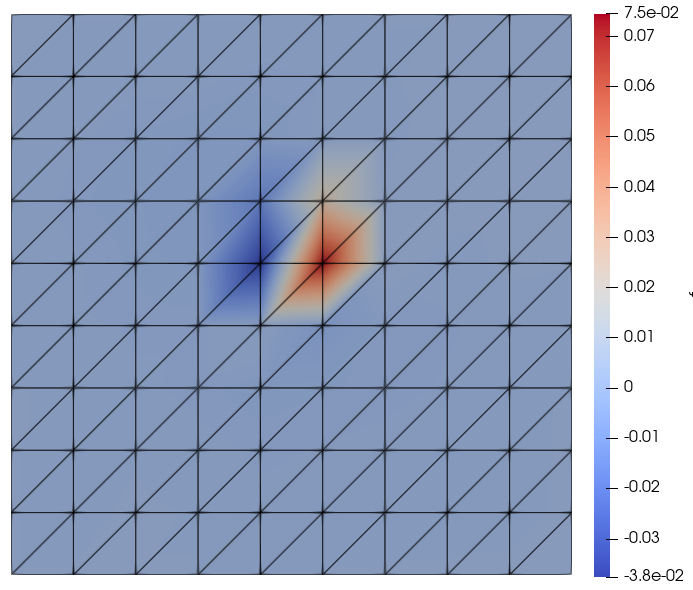
\includegraphics[width=0.2\linewidth]{images/newlines/mesh/explications/addnet/u_theta_h.png}
        \quad
        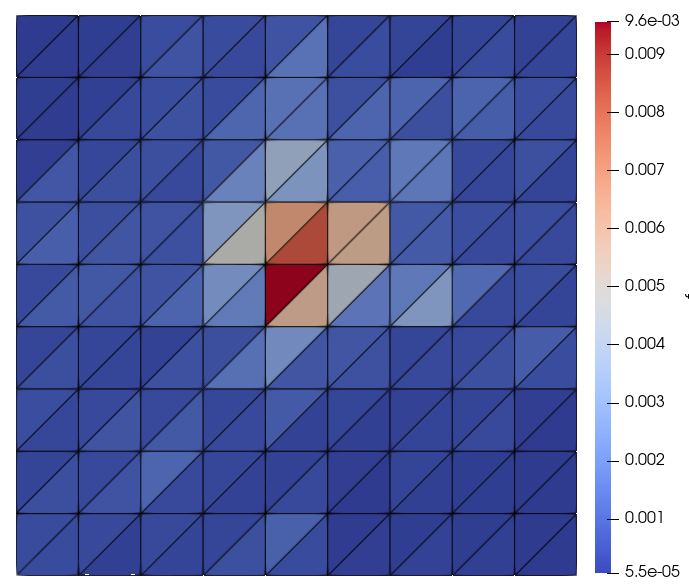
\includegraphics[width=0.2\linewidth]{images/newlines/mesh/explications/addnet/eta_h_addnet.png}
        \quad
        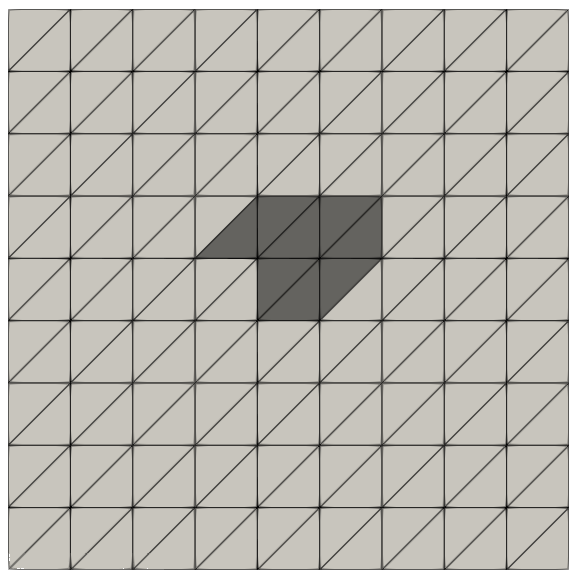
\includegraphics[width=0.17\linewidth]{images/newlines/mesh/explications/addnet/marking_addnet.png}
        \qquad
        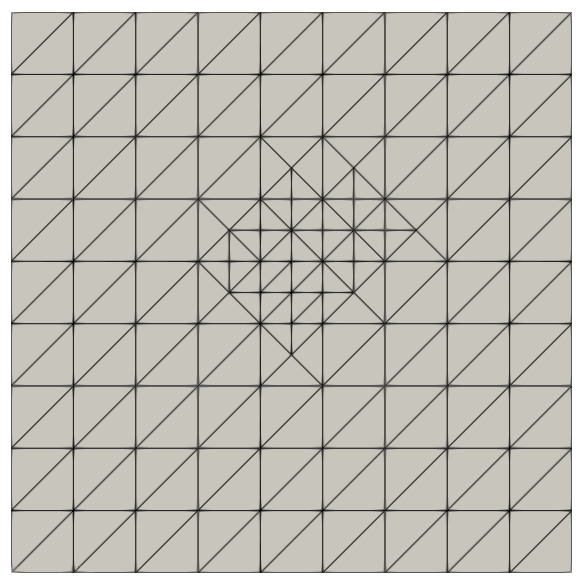
\includegraphics[width=0.17\linewidth]{images/newlines/mesh/explications/addnet/refined_addnet.png}
    \end{center}

    \vspace{-10pt}
    $\cdots\longrightarrow
    \textcolor{red}{\text{INTERPOLATE}}\longrightarrow\hspace{6pt}
    \text{ESTIMATE}\hspace{8pt}\longrightarrow\hspace{14pt}
    \text{MARK}\hspace{14pt}\longrightarrow\hspace{8pt}
    \text{REFINE}\hspace{4pt}\longrightarrow\hspace{1pt}
    \cdots$

    \hspace{55pt}$\textcolor{red}{u_\theta}\hspace{55pt}\eta_{res,T}$

    \vspace{8pt}
    \textbf{Local residual estimator (in $L^2$ norm):} Let $T$ be a cell of $\mathcal{T}_h$ .

    \vspace{-8pt}
    $$\eta_{res,T}^2 = h_T^4 \|\textcolor{red}{(\Delta u_\theta)_h + f_h}\|_{L^2(T)}^2$$
    with $h_\bullet$ the size of $\bullet$ and considering the Poisson problem.
\end{frame}

\begin{frame}{Numerical results}
    \vspace{-10pt}
    \begin{center}
        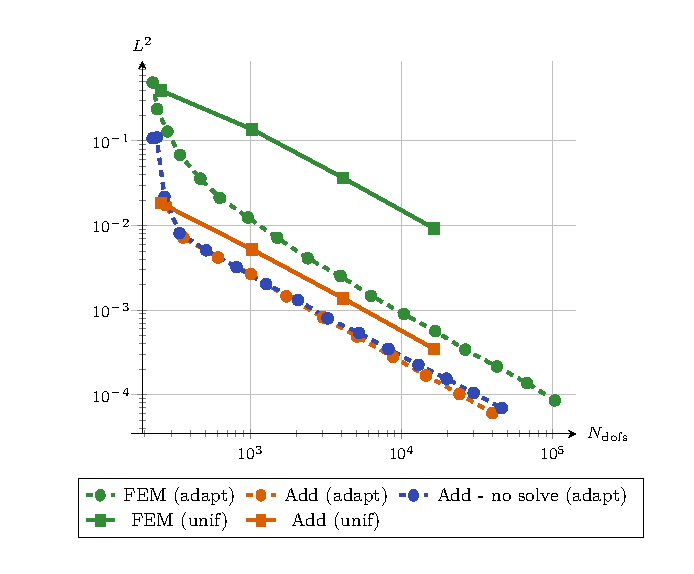
\includegraphics[width=0.4\linewidth]{images/newlines/mesh/results/cvg.pdf}
        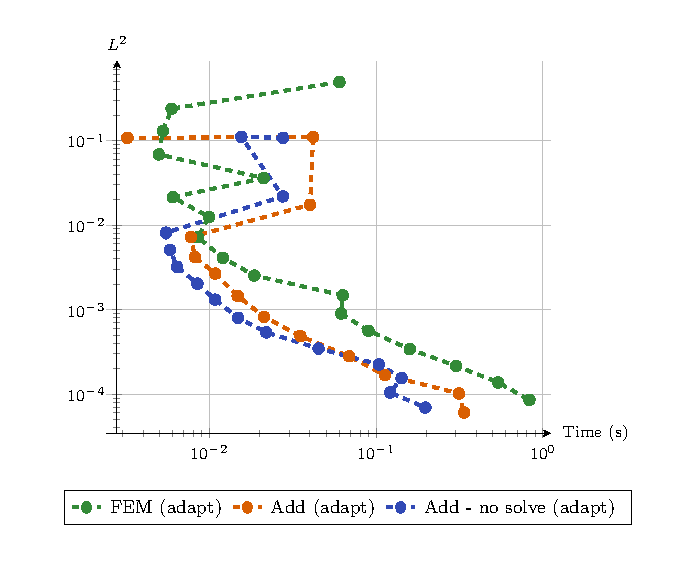
\includegraphics[width=0.4\linewidth]{images/newlines/mesh/results/times.pdf}
    \end{center}
    
    \vspace{-10pt}
    \footnotesize
    \warning \quad Results obtained on a laptop GPU (probably due to external factors).
    
    \normalsize
    \vspace{5pt}
    \textbf{Ideas for improving results :} Additive approach (no resolution).

    \vspace{3pt}
    \begin{minipage}{0.1\linewidth}
        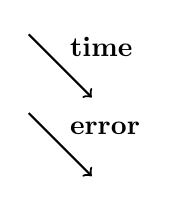
\begin{tikzpicture}[scale=1]
            \draw[->, thick] (0,1.8) -- (0.8,1);
            \node[above right] at (0.4,1.4) {\textbf{time}};

            \draw[->, thick] (0,0.8) -- (0.8,0);
            \node[above right] at (0.4,0.4) {\textbf{error}};
        \end{tikzpicture}
    \end{minipage} \hspace{5pt}
    \begin{minipage}{0.86\linewidth}
        \vspace{2pt}
        Interpolate only mesh points added in the refinement process. \\

        \vspace{5pt}
        Use another metric such as curvature, rather than residual error.

        % \vspace{-5pt}
        % $$\Delta u_\theta+f \qquad \ne \qquad u-u_\theta$$
    \end{minipage}
    % \begin{itemize}
    %     \item To improve execution times: \\ 
    %     Interpolate only mesh points added in the refinement process.
    %     % \item Cout du passage sur GPU.
    %     \item To improve the mesh : \\
    %     Use another metric such as curvature, rather than residual error. \\
    %     (The network residual ($\Delta u_\theta+f$) does not match the additive solution (the network error $u-u_\theta$).)

    % \end{itemize}

\end{frame}

\subsection{\filledstar Non linear PDEs}

\begin{frame}{Problem considered}	
    \textbf{Objective:} Extend the additive approach to non linear PDEs.

    \vspace{10pt}
    \textbf{Problem statement:} Considering the \textcolor{red}{non linear Poisson problem with Dirichlet BC}:
    \vspace{-5pt}
    \begin{equation*}
        \left\{
        \begin{aligned}
            -\text{div}\big((1+4u^4)\nabla u\big) & = f, \; &  & \text{in } \; \Omega, \\
            u         & = 1, \;  &  & \text{on } \; \partial\Omega.
        \end{aligned}
        \right.
    \end{equation*}

    with $\Omega=[-0.5\pi,0.5\pi]^2$ and $\mathcal{M}=[-0.5,0.5]^2$ ($p=2$).

    \vspace{5pt}
	\textbf{Analytical solution :}

	\vspace{-12pt}
	\begin{equation*}
		u(\bm{x};\bm{\mu})= 1 + \exp\left(-\frac{(x-\mu_1)^2+(y-\mu_2)^2}{2}\right)\sin(2x)\sin(2y)
	\end{equation*}
	\vspace{-5pt}
	
    \vspace{5pt}
	\textbf{PINN training:} Imposing BC exactly with a level-set function.

\end{frame}

\begin{frame}{Newton method}
    

    We want to solve the non linear system: \hfill \tiny $N_h$ : number of degrees of freedom.

    \normalsize
    \vspace{-10pt}
    \begin{equation}
        \label{eq:nonlinear}
        F(u) = 0 
    \end{equation}

    \vspace{-2pt}
    with $F:\mathbb{R}^{N_h} \to \mathbb{R}^{N_h}$ a non linear operator and $u\in\mathbb{R}^{N_h}$ the unknown vector.

    \begin{center}
        \small
        \begin{minipage}{0.9\linewidth}
            \begin{algorithm}[H]
                \SetAlgoLined
                \caption{Newton's method to solve \eqref{eq:nonlinear} \citep{newton_accel_2025}}
                \textbf{Initialization step:} set $u^{(0)} = u_0$\;
                \For{\( k \ge 0 \)}{
                    Solve the linear system \( F(u^{(k)}) + F'(u^{(k)}) \delta^{(k+1)} = 0 \) for \( \delta^{(k+1)} \)\;
                    Update \( u^{(k+1)} = u^{(k)} + \delta^{(k+1)} \)\;
                }
            \end{algorithm}
        \end{minipage}
    \end{center}

    \vspace{5pt}
    \textbf{Standard version:} \\
    Initialization with a constant value $u_0$. For instance, $u_0=1$.

    \vspace{5pt}
    \textbf{DeepPhysics version:} \citep{odot_deepphysics_2021} \\
    Initialization with a PINN solution $u_0=u_\theta$.
\end{frame}

\begin{frame}[noframenumbering]{Newton method}
    \vspace{5pt}
    We want to solve the non linear system: \hfill \tiny $N_h$ : number of degrees of freedom.

    \normalsize
    \vspace{-10pt}
    \begin{equation}
        F(u) = 0 \tag{1}
    \end{equation}

    \vspace{-2pt}
    with $F:\mathbb{R}^{N_h} \to \mathbb{R}^{N_h}$ a non linear operator and $u\in\mathbb{R}^{N_h}$ the unknown vector.

    \begin{center}
        \small
        \begin{minipage}{0.9\linewidth}
            \begin{algorithm}[H]
                \SetAlgoLined
                \caption{\textcolor{red}{Additive approach} to solve \eqref{eq:nonlinear} }
                \textbf{Initialization step:} set \textcolor{red}{$p_+^{(0)} = 0$}\;
                \For{\( k \ge 0 \)}{
                    Solve the linear system \( F(\textcolor{red}{p_+^{(k)}+u_\theta}) + F'(\textcolor{red}{p_+^{(k)}+u_\theta}) \delta^{(k+1)} = 0 \) for \( \delta^{(k+1)} \)\;
                    Update \( \textcolor{red}{p_+^{(k+1)}} = \textcolor{red}{p_+^{(k)}} + \delta^{(k+1)} \)\;
                }
            \end{algorithm}
        \end{minipage}
    \end{center}

    \textbf{Advantage compared to DeepPhysics:}

    \begin{center}
    $u_\theta$ is not required to live in the same space as $p_h^+$.
    \end{center}
\end{frame}

\begin{frame}{Numerical results}	
    \vspace{-10pt}
    \begin{center}
        \begin{minipage}{0.58\linewidth}
            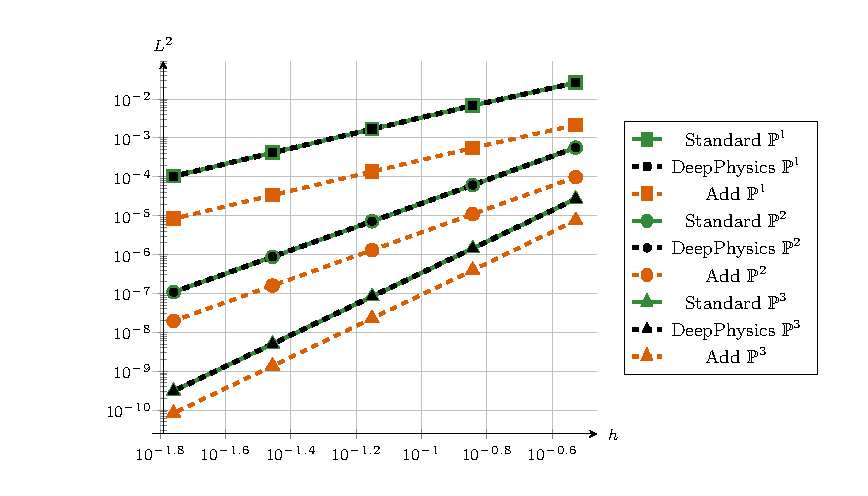
\includegraphics[width=\linewidth]{images/newlines/nonlinear/results/cvg_cropped.pdf}
        \end{minipage}
        \begin{minipage}{0.38\linewidth}
            \small
            \textbf{Number of iterations :}

            \begin{itemize}
                \item Standard Newton: $8$ iterations.
                \item DeepPhysics: $4$ iterations.
                \item Additive approach: $4$ iterations.
            \end{itemize}
        \end{minipage}
        
        \vspace{-10pt}
        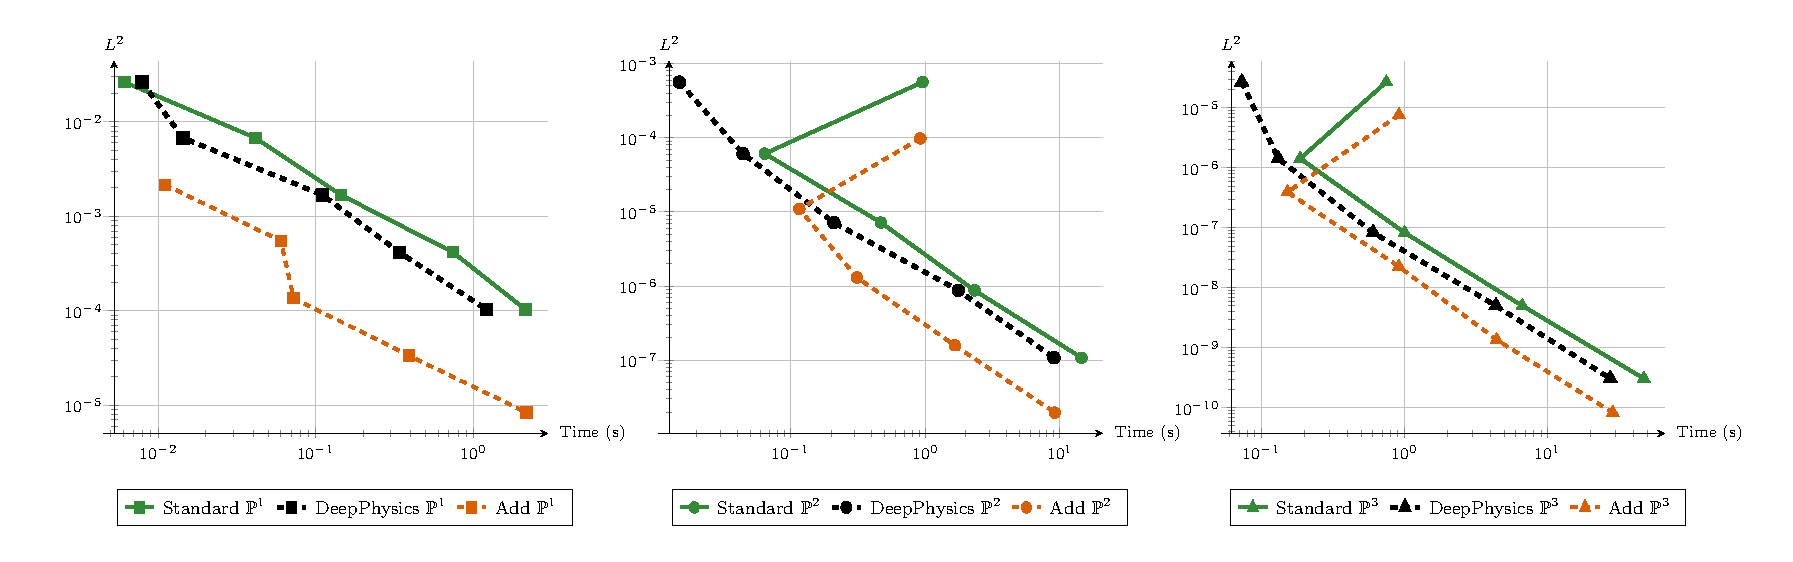
\includegraphics[width=\linewidth]{images/newlines/nonlinear/results/times_cropped.pdf}
    \end{center}
\end{frame}